\documentclass{standalone}
\usepackage{tikz}
\usetikzlibrary{positioning,shapes,shadows,arrows}

\begin{document}
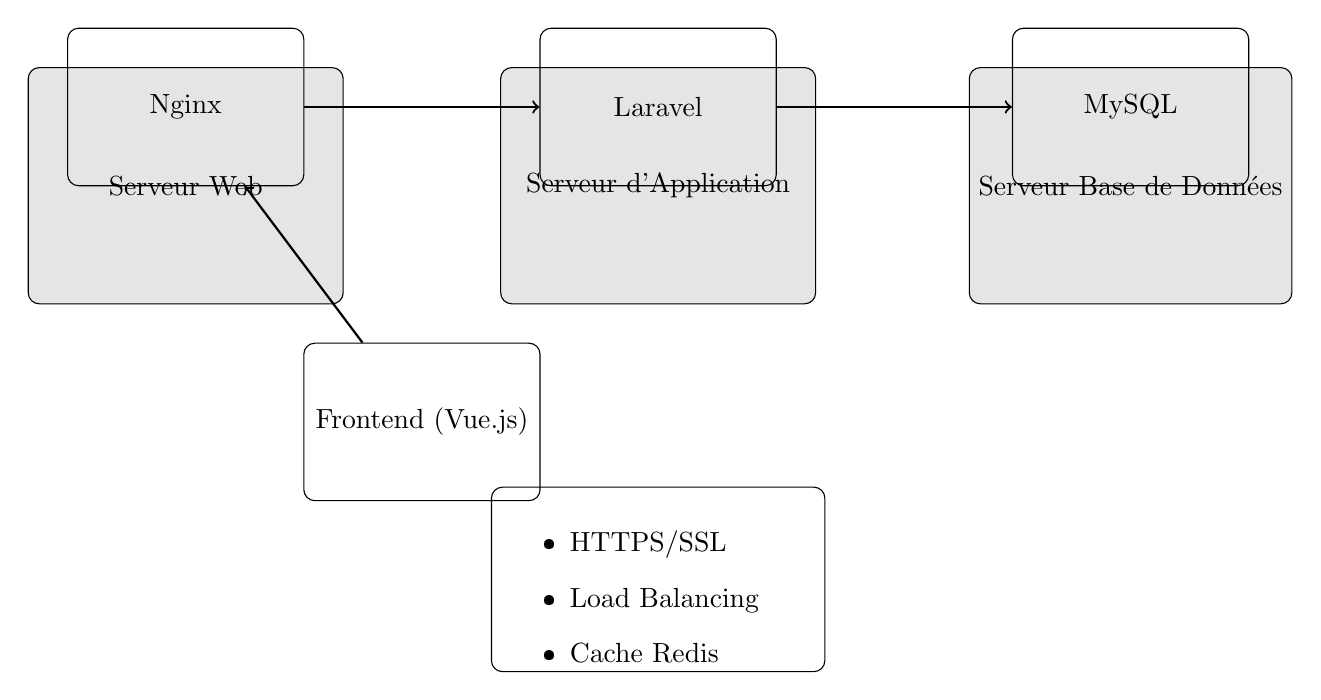
\begin{tikzpicture}[
    node/.style={draw, rectangle, rounded corners, minimum width=3cm, minimum height=2cm},
    server/.style={draw, rectangle, rounded corners, minimum width=4cm, minimum height=3cm, fill=gray!20},
    arrow/.style={->, thick}
]

% Servers
\node[server] (web_server) at (0,0) {Serveur Web};
\node[server] (app_server) at (6,0) {Serveur d'Application};
\node[server] (db_server) at (12,0) {Serveur Base de Données};

% Components
\node[node] (nginx) at (0,1) {Nginx};
\node[node] (laravel) at (6,1) {Laravel};
\node[node] (mysql) at (12,1) {MySQL};

% Frontend
\node[node] (frontend) at (3,-3) {Frontend (Vue.js)};

% Connections
\draw[arrow] (nginx) -- (laravel);
\draw[arrow] (laravel) -- (mysql);
\draw[arrow] (frontend) -- (nginx);

% Notes
\node[draw, rectangle, rounded corners, text width=4cm] at (6,-5) {
    \begin{itemize}
        \item HTTPS/SSL
        \item Load Balancing
        \item Cache Redis
    \end{itemize}
};

\end{tikzpicture}
\end{document} 